\section{Geradlinige Dreiecks Darstellungen (SLTRs)}

Ausgehend von den konvexen Einbettungen nach Tutte, könnte man sich die Frage stellen, unter welchen Vorraussetzungen wir einen planaren Graphen so zeichnen können, dass alle Gebiete ein bestimmtes Polygon umranden. Wir werden dieser Frage im Fall von Dreiecken nachgehen. Die Formalisierung dieser Darstellung und erste Folgerungen folgen Nieke Aerts und Stefan Felsner \cite{af13,af15}.

\begin{definition}[SLTR]\label{defsltr}
Eine Zeichnung eines planen Graphen $G$ wird \textit{geradlinige Dreiecksdarstellung}, im weiteren kurz \textit{SLTR} (für die englische Bezeichnung \textit{staight line triangle representation}), genannt falls gilt:
\begin{itemize}
\item[S1] Alle Kanten sind Segmente von Geraden.
\item[S2] Alle Gebiete, inklusive dem Äusseren, sind nicht degenerierte Dreiecke.
\end{itemize}
\end{definition}

\begin{figure}[h]
	\centering
  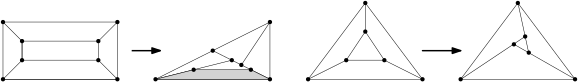
\includegraphics[width=0.8\textwidth]{sltr-example.png}
	\caption{Links einer der beiden 3-zusammenhängenden Graphen auf acht Knoten ohne SLTR und rechts ein Graph mit einer möglichen SLTR.}
\end{figure}

Um die Problemstellung greifbarer zu machen kann man plane Graphen zusammen mit den Aufhängungen $\{a_1,a_2,a_3\}$ betrachten, wobei $a_1,a_2$ und $a_3$ die designierten Ecken des äusseren Gebietes einer möglichen SLTR sind. Einen Graphen zusammen mit einem äusseren Gebiet beziehungsweise festen Aufhängungen als Paar zu behandeln ist sinnvoll. Es existieren planare Graphen, von denen manche Einbettungen SLTRs zulassen, andere jedoch nicht, so wie in Abbildung \ref{10_example} zu sehen. Für intern-3-zusammenhängende planare Graphen ist die topologische Einbettung (und somit die Gebiete von $G$) nach der Auswahl der Aufhängungen eindeutig. Die nächste Präposition enthält eine erste notwendige Bedingung für die Existenz von geradlinigen Dreiecksdarstellungen.

\begin{proposition}\cite[Proposition 1.2]{af13}
Sei $G$ ein planer Graph mit den Aufhängungen $\{a_1,a_2,a_3\}$ als äussere Ecken einer SLTR. Weiter gebe es keine inneren Knoten $v$ mit $deg(v) < 3$. Dann ist $G$ intern-3-zusammenhängend.
\end{proposition}

\begin{proof}
Sei $\Delta$ die SLTR von $G=(V,E)$. Angenommen es existiert eine Menge $U \subseteq V$ in $G$ mit $|U| = 2$, deren Entnahme $G$ in nicht zusammenhängende Komponenten trennt. Wir werden zeigen, dass jeder Teil von $G\backslash U$ eine der Aufhängungen enthält und somit $G + v_\infty$ nicht von $U$ getrennt wird. Jeder innerer Knoten in $G$ hat Grad grösser als zwei. Sei $K$ eine der Komponenten von $G\backslash U$, und sei $P$ ein Pfad der entsteht wenn wir $U$ wieder einfügen. Dann muss $K$ eine Aufhängung enthalten.

Falls $U$ keinen Pfad induziert, dann betrachte die konvexe Hülle von $U \cup K$ in $\Delta$. Mindestens drei der Ecken von $U \cup K$ haben Aussenwinkel grösser als $\pi$. Zwei dieser Winkel können an den Knoten aus $U$ liegen, aber der dritte muss ein Winkel sein der schon in $\Delta$ existiert. Es handelt sich somit um eine Aufhängung.


\end{proof}

\begin{remark}
Für innere Knoten von Grad 2 in einer SLTR müssen beide angrenzenden Winkel gerade sein. Somit kann man diese Knoten durch eine gerade Kante zwischen ihren Nachbarn ersetzen und den resultierenden Graphen betrachten. Wir werden somit von nun an nur intern-3-zusammenhängende Graphen mit Aufhängungen betrachten, da alle anderen Graphen, die eine SLTR zulassen, auf diese reduziert werden können.
\end{remark}

\begin{figure}[h]
	\centering
  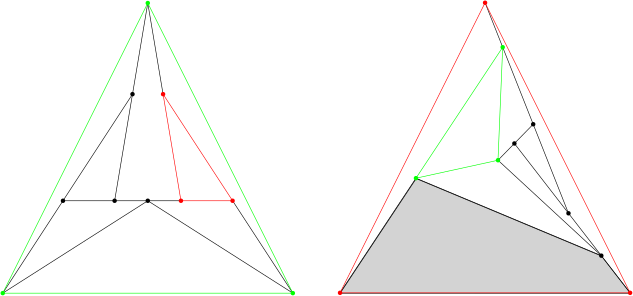
\includegraphics[scale=0.1]{10_example.png}
	\caption{Der kleinste 3-zusammenhängende kombinatorische Graph mit einer Wahl der Aufhängungen die eine SLTR zulässt und einer Auswahl ohne SLTR.}
	\label{10_example}
\end{figure}

Zu den Fragen, welche notwendigen und hinreichenden Bedingungen es für die Existenz von SLTRs gelten und  welche algorithmischen Ansätze man bei der Suche nach einer spezifischen Darstellung verfolgen kann, haben Aerts und Felsner in \cite{af13}, \cite{af13h} und \cite{af15} schon einige Antworten geliefert. Die nächsten zwei Kapitel, werden sich mit diesen auseinandersetzen. 

Zuvor werden in diesem Kapitel noch einige notwendige Konzepte eingeführt, die notwendig sind um der Argumentation zu folgen.
